% clashbot final report, CAP 6938 AI Knowledge Systems (UCF), IEEE two-column conference format.
% Compile: tectonic -X compile clashbot_report.tex   (or pdflatex + bibtex + pdflatex x2 on Overleaf)
%
% Source convention: every number carries a "% src:" comment naming the file it was copied from.
%   CMA = docs/research/course_mapping_audit.md       PBA = docs/research/packaging_and_benchmarks_audit.md
%   PBC = docs/research/prior_bots_comparison.md      CGA = docs/research/course_gap_analysis.md
%   BM  = docs/data/BENCHMARKS.md   SA = docs/data/stats_audit_v1.md   STATUS = docs/mac/STATUS.md
%   D-nnn = docs/decisions/DECISIONS.md   CC = docs/data/context_conflict_v1.md   AR = docs/data/answer_rules_v1.md
%   VP = docs/data/vs_pro_v1.md   LAT = docs/data/latency_v2.md
% Revision 2 (2026-11-07): every number once tagged [pre-merge] was re-checked against the merged docs/data
% files (MAC-AP, MAC-AR) and the tag removed.
% Revision 3 (2026-11-07 night): vs_pro_v1 is final (all 24 usable test games, generated 2026-11-08T02:31:35Z); the
% Training Camp trial is filled. TRIAL = the user's recorded results of the 10 trial battles (2026-11-07 evening,
% scripts/demo.sh --live, frozen code D-051) as relayed for revision 3; LOG = session log runs/demo/20261107-213709
% (battles.jsonl, decisions.jsonl; 9 of 10 battles logged); BL = docs/plans/BACKLOG_post_showcase.md (W1-W12).
% No placeholders remain.

\documentclass[conference]{IEEEtran}
\usepackage{iftex}
\ifXeTeX % local tectonic builds: Times-compatible fonts so the page count matches pdflatex on Overleaf
  \usepackage{fontspec}
  \setmainfont{texgyretermes}[Extension=.otf, UprightFont=*-regular, BoldFont=*-bold,
    ItalicFont=*-italic, BoldItalicFont=*-bolditalic]
  \setsansfont{texgyreheros}[Extension=.otf, UprightFont=*-regular, BoldFont=*-bold,
    ItalicFont=*-italic, BoldItalicFont=*-bolditalic]
  \setmonofont{texgyrecursor}[Extension=.otf, UprightFont=*-regular, BoldFont=*-bold,
    ItalicFont=*-italic, BoldItalicFont=*-bolditalic]
\fi
\usepackage{cite}
\usepackage{amsmath,amssymb}
\usepackage{graphicx}
\usepackage{booktabs}
\usepackage{array}
\usepackage{xcolor}
\usepackage{url}
\usepackage{tikz}
\usetikzlibrary{arrows.meta}
\usepackage[hidelinks]{hyperref}

\newcommand{\cb}{\textsc{clashbot}}
\newcommand{\tw}[1]{\texttt{#1}}
\newcolumntype{L}[1]{>{\raggedright\arraybackslash}p{#1}}

\begin{document}

\title{\cb{}: A Knowledge-Grounded LLM Agent That Plays Clash Royale in Real Time from Pixels}

\author{\IEEEauthorblockN{David Tyler Jackson (5298477)}
\IEEEauthorblockA{CAP 6938 AI Knowledge Systems, University of Central Florida\\
Instructor: Dr.\ Ser Nam Lim}}

\maketitle

\begin{abstract}
% src: CMA C1 (197 games, 10,923 states), C2 (KG v2 840/27,112), LOG (323 ms trial-session p50); SA sec. 1 (0.507, 0.482, 0.384); CC (E2); AR (E6); STATUS 2026-11-07 night (first win)
We present \cb{}, a non-embedded agent that plays the real-time card game Clash Royale on an iPhone through macOS screen mirroring, with pixels in and taps out and every model running on one laptop. A fast loop runs YOLOv8 detection, OCR and tracking, a learned play/wait gate, and a candidate generator built from a tactical lane simulator, hybrid retrieval over 10,923 states from 197 pro games, and a knowledge graph of 840 nodes and 27,112 edges. A 600M-parameter decision LLM, fine-tuned on the pro games, chooses one of at most four candidates and remains the decision maker. On held-out games it picks the pro's play 50.7\% of the time (95\% CI 47.2--54.0) among four hard options, against 25\% chance and 38.4\% for a placement prior. Three negative results are findings in their own right: a tuned LightGBM ranker (48.2\%) is statistically indistinguishable from the LLM; removing, shuffling or poisoning the tool notes in the LLM's context leaves its accuracy unchanged; and answer rules mined from the pro games beat random but not card popularity. Run open loop on 24 held-out pro games, the bot acts within 2\,s of 77.1\% of the pro's plays but picks the pro's card on only 17.1\% of them, largely because the pro's card is in its perceived hand only 40\% of the time. % src: VP headline (77.1, 17.1, 40.1)
In the live trial session a decision takes 323\,ms from capture to click at the median. The agent won one Training Camp battle in an early session but lost all ten battles of a trial on the frozen code (95\% CI for the win rate 0--30.8\%, no different from the prior agent KataCR's 1/20), so it does not yet beat Training Camp reliably; its logs trace the losses to unstable tower-HP reading, no committed target tower, weak spell valuation and over-playing. % src: TRIAL; STATUS 2026-11-07 night (win in run 013441); BL W1, W2, W5, W8
\end{abstract}

\begin{IEEEkeywords}
game agents, knowledge graphs, retrieval-augmented decision making, LLM ranking, real-time systems
\end{IEEEkeywords}

% ---------------------------------------------------------------------------------------------
\section{Introduction}

Clash Royale is a real-time, two-player card game played on phones. Each player brings a hidden deck of eight cards, holds four of them, and spends elixir, which regenerates up to ten, to place troops, buildings and spells on an 18$\times$32-tile arena; a match lasts three minutes plus up to two minutes of overtime~\cite{wu2025nonembedded}. % src: PBC sec. 1.1 (deck 8, hand 4, 3 + 2 min, 18 x 32 grid)
\cb{} is a \emph{non-embedded} agent~\cite{wu2025nonembedded}: it has no game API, reads the screen of an iPhone mirrored onto a Mac, and acts by clicking the mirrored window, the interface a human uses.

The task is hard for five measurable reasons. (i)~\emph{Real time}: perception runs on a stream with a 10\,fps target (7.97\,fps reached in live run 111554) and capture to click takes 323\,ms at the median in the live trial session. % src: LOG (323 ms); CMA C7 (7.97 fps, run 20261107-111554)
(ii)~\emph{Partial, noisy observation}: the opponent's deck, hand and elixir are hidden, and our own reading of the board is imperfect; the pro's recorded move passes our perceived-legality check on only 0.542--0.597 of states. % src: CMA A3 neuro-symbolic row (ranker_stats_v1.json pos_in_legal_rate)
(iii)~\emph{A structured action space plus a timing decision}: an action is card $\times$ lane $\times$ zone or hold (D-010), and pros deploy within the next second on about a fifth of seconds (dense act rate 0.204). % src: CMA B dense wait/act row
(iv)~\emph{Sparse supervision}: the expert data are 197 pro games (about 12 match-hours, one creator) with no reward and no simulator, and the Training Camp opponent plays level-15 cards. % src: CMA C1; D-047
(v)~\emph{Consumer hardware}: everything runs on an Apple M5 laptop with 32\,GB and no paid API. % src: CMA C3 (hardware); PBC sec. 4 (cost per game)

The design follows the course's retrieve-then-rank and agent-with-tools patterns~\cite{lim2026l11,lim2026l13,lim2026l15}. Deterministic tools (a tactical engine with a lane simulator, hybrid retrieval over pro states, and a knowledge graph) propose at most four candidate plays with short text notes; a decision LLM fine-tuned on the pro games picks one. By project decision the LLM stays the decision maker and no tool picks the move (D-045; design decisions are logged in the repository as D-001 to D-053). Our contributions:
\begin{enumerate}
\item A non-embedded, two-speed agent that plays live through iPhone Mirroring with all models local (Sec.~\ref{sec:system}).
\item A knowledge layer: retrieval over 10,923 pro states (644-d structured vector and BM25, fused by RRF), a two-version knowledge graph with lane-simulation edges and 3,620 mined pro answers, and a tactical engine, all rendered as context for a fine-tuned setwise LLM ranker. % src: CMA C1, C2, A1
\item A leakage-checked benchmark suite. Our first multiple-choice options leaked the answer (a rule reading only option keys scored 0.852 on test); we rebuilt them as a 2$\times$2 card$\times$placement grid and compare ten rankers with cluster-bootstrap CIs, plus ablations for retrieval, KG embeddings, mined rules, context conflict, timing, next-card prediction and knowledge editing, and an open-loop comparison with the pro on held-out videos, negative results included (Sec.~\ref{sec:exp}). % src: D-037 (0.852 test)
\item Live evaluation in Training Camp: 13 recorded runs (931 logged decisions) with one win, then a 10-battle trial on the frozen code that the bot lost 0--10 (95\% CI 0--30.8\%; KataCR 1/20, Fisher $p=1.0$), and a diagnosis of the losses from the logs (Sec.~\ref{sec:live}, \ref{sec:disc}). % src: CMA C6; STATUS 2026-11-07 night; TRIAL; BL
\item Demo tooling: a launcher that taps only when the opponent banner reads ``Trainer'', behind a two-switch live guard, and a decision dashboard (Fig.~\ref{fig:dashboard}).
\end{enumerate}
The bot plays only Training Camp and friendly battles, never ranked matches against people (D-031, D-050).

% ---------------------------------------------------------------------------------------------
\begin{figure*}[t]
\centering
\resizebox{\textwidth}{!}{%
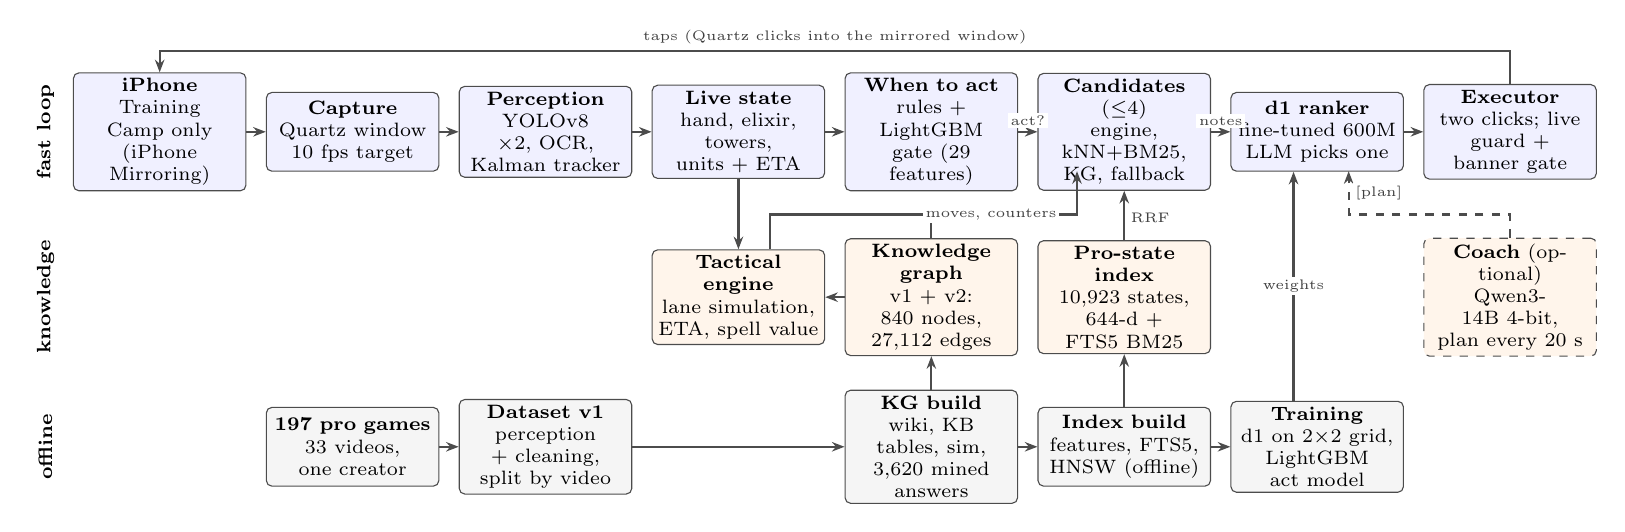
\begin{tikzpicture}[
  box/.style={draw=black!70, rounded corners=2pt, align=center, font=\scriptsize,
              text width=2.05cm, minimum height=1.0cm, inner sep=2pt, fill=white},
  fast/.style={box, fill=blue!6},
  know/.style={box, fill=orange!8},
  off/.style={box, fill=black!4},
  arr/.style={-{Stealth[length=1.6mm]}, thick, draw=black!70},
  lab/.style={font=\tiny, text=black!75, fill=white, inner sep=1pt}]
% row 1: fast loop
\node[fast] (phone) at (0,0)     {\textbf{iPhone}\\Training Camp only\\(iPhone Mirroring)};
\node[fast] (cap)   at (2.45,0)  {\textbf{Capture}\\Quartz window\\10 fps target};
\node[fast] (per)   at (4.9,0)   {\textbf{Perception}\\YOLOv8 $\times$2, OCR,\\Kalman tracker};
\node[fast] (st)    at (7.35,0)  {\textbf{Live state}\\hand, elixir, towers,\\units + ETA};
\node[fast] (gate)  at (9.8,0)   {\textbf{When to act}\\rules + LightGBM\\gate (29 features)};
\node[fast] (cand)  at (12.25,0) {\textbf{Candidates} ($\le$4)\\engine, kNN+BM25,\\KG, fallback};
\node[fast] (d1)    at (14.7,0)  {\textbf{d1 ranker}\\fine-tuned 600M\\LLM picks one};
\node[fast] (ex)    at (17.15,0) {\textbf{Executor}\\two clicks; live\\guard + banner gate};
% row 2: knowledge layer
\node[know] (eng)   at (7.35,-2.1)  {\textbf{Tactical engine}\\lane simulation,\\ETA, spell value};
\node[know] (kg)    at (9.8,-2.1)   {\textbf{Knowledge graph}\\v1 + v2: 840 nodes,\\27,112 edges};
\node[know] (idx)   at (12.25,-2.1) {\textbf{Pro-state index}\\10,923 states,\\644-d + FTS5 BM25};
\node[know, dashed] (coach) at (17.15,-2.1) {\textbf{Coach} (optional)\\Qwen3-14B 4-bit,\\plan every 20 s};
% row 3: offline
\node[off] (vid)    at (2.45,-4.0)  {\textbf{197 pro games}\\33 videos,\\one creator};
\node[off] (ds)     at (4.9,-4.0)   {\textbf{Dataset v1}\\perception + cleaning,\\split by video};
\node[off] (kgb)    at (9.8,-4.0)   {\textbf{KG build}\\wiki, KB tables, sim,\\3,620 mined answers};
\node[off] (idxb)   at (12.25,-4.0) {\textbf{Index build}\\features, FTS5,\\HNSW (offline)};
\node[off] (tr)     at (14.7,-4.0)  {\textbf{Training}\\d1 on 2$\times$2 grid,\\LightGBM act model};
% row labels
\node[font=\scriptsize\bfseries, rotate=90] at (-1.45,0)    {fast loop};
\node[font=\scriptsize\bfseries, rotate=90] at (-1.45,-2.1) {knowledge};
\node[font=\scriptsize\bfseries, rotate=90] at (-1.45,-4.0) {offline};
% fast-loop arrows
\draw[arr] (phone) -- (cap);
\draw[arr] (cap) -- (per);
\draw[arr] (per) -- (st);
\draw[arr] (st) -- (gate);
\draw[arr] (gate) -- node[lab, above=1pt] {act?} (cand);
\draw[arr] (cand) -- node[lab, above=1pt] {notes} (d1);
\draw[arr] (d1) -- (ex);
\draw[arr] (ex.north) -- ++(0,0.42) -| node[lab, pos=0.25, above=1pt] {taps (Quartz clicks into the mirrored window)} (phone.north);
% knowledge-layer arrows
\draw[arr] (st.south) -- (eng.north);
\draw[arr] (kg.west) -- (eng.east);
\draw[thick, draw=black!70] (kg.north) -- (9.8,-1.05);
\draw[arr] ([xshift=4mm]eng.north) |- (11.65,-1.05) -- node[lab, pos=0.0, left=6pt] {moves, counters} (11.65,-0.5);
\draw[arr] (idx.north) -- node[lab, right=1pt, pos=0.45] {RRF} (cand.south);
\draw[arr, dashed] (coach.north) |- (15.1,-1.05) -- node[lab, pos=0.5, right=1pt] {[plan]} (15.1,-0.5);
% offline arrows
\draw[arr] (vid) -- (ds);
\draw[arr] (ds) -- (kgb);
\draw[arr] (kgb) -- (idxb);
\draw[arr] (idxb) -- (tr);
\draw[arr] (kgb) -- (kg);
\draw[arr] (idxb) -- (idx);
\draw[arr] ([xshift=-3mm]tr.north) -- node[lab, pos=0.5] {weights} ([xshift=-3mm]d1.south);
\end{tikzpicture}}
\caption{Two-speed architecture (D-007). The fast loop runs on every decision (323\,ms p50 capture to click in the live trial); tools in the knowledge layer only propose candidates and write notes, the fine-tuned d1 LLM picks the move (D-045). The coach is optional and off by default. Every decision is logged and can be replayed in the dashboard (Fig.~\ref{fig:dashboard}).}
\label{fig:pipeline}
\end{figure*}
% src (figure numbers): LOG (323 ms), C2 (840 / 27,112), C1 (197 games, 33 videos, 10,923 x 644), C3/B (Qwen3-14B coach, 20 s period), act_gbdt_v1.md (29 features), CMA C2 extras (3,620 answers)

% ---------------------------------------------------------------------------------------------
\section{Related Work}

\emph{Game agents.} AlphaStar~\cite{vinyals2019alphastar} and OpenAI Five~\cite{berner2019dota} reached expert level through game APIs and large-scale self-play, which a phone game without an API does not offer. KataCR~\cite{wu2025nonembedded} is the closest work: a non-embedded Clash Royale agent with YOLOv8 detectors, OCR and an offline-RL StARformer policy in the Decision Transformer formulation~\cite{chen2021dt}, which won 1 of 20 Training Camp games (Table~\ref{tab:prior}). We reuse its detector weights~\cite{wu2024katacr} and its Training Camp protocol. Claude Royale~\cite{houseworth2025claudeRoyale} puts Claude Haiku agents in the loop at about 7\,s per decision, on the human ladder. % src: PBC sec. 1.3, 2.1, 2.2

\emph{LLM agents and ranking.} ReAct, Reflexion and LATS~\cite{yao2023react,shinn2023reflexion,zhou2024lats} spend seconds per step on reasoning, reflection or search. A real-time budget rules out generation in the fast loop, so our LLM acts as a setwise reranker~\cite{zhuang2024setwise,sun2023rankgpt} over tool proposals, as in two-stage recommender serving~\cite{yi2019twotower,lim2026l13}. Fine-tuning an LM to choose among items follows TALLRec and P5~\cite{bao2023tallrec,geng2022p5}; putting graph facts in the context follows GraphRAG~\cite{edge2024graphrag}; deciding when to consult the model follows adaptive retrieval~\cite{jiang2023flare,jeong2024adaptiverag}.

% ---------------------------------------------------------------------------------------------
\section{System}
\label{sec:system}

\subsection{Overview}
Fig.~\ref{fig:pipeline} shows the two-speed design (D-007). The fast loop runs capture, perception, a clean live state, a play/wait gate, candidate generation, the d1 ranker and the executor. An optional slow loop (Qwen3-14B, 4-bit~\cite{qwen2025qwen3}) rewrites a three-line plan every 20 game seconds in quiet moments; it never picks a move and was used in one live run (21 plans, 5.98/6.86\,s p50/p95). The default live path calls no generative LLM. % src: CMA B coach row (run 20261106-133529)

\subsection{Perception and live state}
Frames come from the iPhone Mirroring window by Quartz window capture (632$\times$1392 pixels, 22--38\,ms per grab). % src: STATUS 2026-11-03 Wave 4
Two YOLOv8 detectors~\cite{jocher2023yolov8} with KataCR's published weights~\cite{wu2024katacr} (87.8\,MB each) run on the M5 GPU at 100.5\,ms per call; RapidOCR~\cite{rapidai2021rapidocr} reads the clock and deploy labels on a background worker; a template matcher reads the four hand slots (33.1\,ms) and is re-run only when a slot crop changes (D-038); a Kalman tracker~\cite{kalman1960} follows units. % src: CMA C3, C7
The live-state builder turns detections into own and opponent elixir, hand, towers, the opponent's seen cards and each unit's time to reach a tower (ETA). Computing ETA from the card's speed and attack range instead of the raw track cut its median absolute error from 1.49\,s to 0.30\,s and raised the share within 1\,s from 34\% to 80\% (384 frames, 11 arrivals, one video). % src: docs/data/eta_eval_v1.md (= runs/smoke/AL/eta.md; BM sec. 10)
The same builder produced the dense training data (D-040), so the play/wait model sees the same features live and offline.

\subsection{Data pipeline}
A scraper built a knowledge base from the Clash Royale wiki; then 197 games from 33 videos of one professional creator were perceived and cleaned into 10,923 states (6,901 plays, 3,539 key moments, 483 periodic samples). Bad fields are repaired and flagged, never deleted (D-011); for example, 2,165 states have an unknown placement. % src: README.md (Phase 1, scraper); CMA C1 (MANIFEST, CLEANING_REPORT_v1.md)
Splits are by video (SHA-1 order, 70/15/15), so no game appears in two splits, the contamination concern raised for RETRO~\cite{borgeaud2022retro}. A second pass re-perceived all 33 videos at one state per second (about 17\,h on the M5) for play/wait labels: does the pro deploy within the next second? % src: CMA C1, A2 RETRO row; PBA 1.2 (17 h)
Table~\ref{tab:data} gives the sizes.

\begin{table}[t]
\caption{Data and knowledge stores (train / val / test where split).}
\label{tab:data}
\centering\footnotesize
\setlength{\tabcolsep}{4pt}
\begin{tabular}{@{}lr@{}}
\toprule
Pro games / videos (one creator) & 197 / 33\\
Videos by split & 23 / 5 / 5\\
Games by split & 142 / 27 / 28\\
States by split & 7,693 / 1,574 / 1,656\\
4-way ranker lines & 3,641 / 761 / 766\\
Dense play/wait lines (one per second) & 29,036 / 5,560 / 5,279\\
Pro-advice documents & 3,654\\
\midrule
KG v1: nodes / edges / relations & 590 / 12,030 / 12\\
KG v2: nodes / edges / relations & 840 / 27,112 / 19\\
\quad lane-simulation edges (STOPS, KILLS, PULLS) & 8,951\\
\quad mined answer events $\rightarrow$ answer rules & 3,620 $\rightarrow$ 287\\
\quad situations / sequences / per-level stat rows & 234 / 450 / 1,734\\
\bottomrule
\end{tabular}
\end{table}
% src: CMA C1 (splits, ranker set, dense set, documents), C2 (KG v1/v2 counts, sim 8,951, answers 287, extras)

\subsection{Knowledge graph}
KG v1 (590 nodes, 12,030 edges, 12 relations) holds wiki COUNTERS and SYNERGY relations, deck membership and 129 mined ANSWERED\_BY edges. KG v2 (D-048) adds a game model: per-level stats for 126 cards (1,734 rows, opponents assumed at level 15), 8,951 STOPS, KILLS and PULLS edges computed by the lane simulator, 3,620 mined answer events (the opponent plays $X$; the pro's first defensive play within 8\,s is $Y$) aggregated into 287 rules with held rates, placement offsets and timing, 234 situation nodes, 450 PLAYED\_AFTER sequences, deck co-occurrence, and role-similarity transfer for our cards that have no pro data. An opponent-deck model completes the hidden deck from the cards seen. % src: CMA C2, A3; answer window 8 s: CGA sec. 8, answer_rules_v1.md
Live, the graph supplies the engine's answer prior, pro placement offsets (when $n\ge5$), an elixir reserve for predicted air cards, a counter channel for candidates, and up to three \tw{KG:} lines in d1's context, e.g.\ \tw{KG: archers L15 x2 445hp 164/hit; answers mini-p-e-k-k-a (role of elite-barbarians, n=4), tesla (role of furnace, n=6)}. % src: CMA B (KG v2 facts row, example line); STATUS 2026-11-06 evening

\subsection{Retrieval}
Each state is a 644-d structured vector (3 scalars, 5 phase values, five 120-d card blocks for hand, deck, opponent deck and recent plays of each side, 6 tower, 24 field and 6 threat values) plus a text rendering indexed by SQLite FTS5 BM25~\cite{robertson2009bm25}. Exact dot-product kNN and BM25 lists are fused by reciprocal rank fusion with $k=60$~\cite{cormack2009rrf}, and the neighbours vote for the plays they contain. The vector is hand-built, not a learned bi-encoder~\cite{lim2026l02}. A 384-d bge-small text channel~\cite{xiao2023cpack} and an HNSW index~\cite{malkov2020hnsw} were evaluated but are not on the live path (Sec.~\ref{sec:retr}). % src: CMA A1 (644-d breakdown, RRF k = 60, HNSW offline only, text channel not integrated)

\subsection{Tactical engine}
The engine (1,750 lines; roles for 122 cards) lists enemy pushes, estimates each push's tower damage with a lane simulation over per-level stats, and proposes placed answers with reasons. For example, a lone level-15 Balloon deals 3,162 tower HP unanswered, 351 with a Musketeer behind the tower, and 0 with a Tesla pull. It values spells by kills (a Zap needs at least two kills and value 2.5), leads spells by their flight time, keeps buildings inside a pull box, and tracks elixir trades and offence windows. Its analysis is written as \tw{tactics:} lines and per-option notes, which is how d1 reads it (D-042). % src: CMA B (1,750 lines, 122 cards, balloon 3,162/351/0); STATUS MAC-AM merged (spell bar, lead, tesla box)

\subsection{When to act}
A reactive policy (modes defend, leak, punish, counter, spell, save and none; D-041) holds by default and filters candidates by mode, e.g.\ defend keeps the threat's lane on our half. A LightGBM~\cite{ke2017lightgbm} model on 29 features predicts whether a pro would deploy within 2\,s (threshold 0.47, 0.05\,ms per call). In the live \emph{fast} policy the rules override the model in defend, counter, spell and leak, and save and none always hold. This gate is our adaptive trigger~\cite{jiang2023flare}: it decides when the LLM is consulted at all. % src: CMA sec. 0 (when to act), B (act model 0.045 ms)

\subsection{Candidates and the d1 ranker}
The generator returns at most four plays: up to two engine moves, then retrieval votes, KG v1 counter scores (weight 0.5) and legal fallbacks; the policy, the read hand and a hold rule for fallbacks below 9.5 elixir filter them. % src: CMA sec. 0 (candidates, filters)
d1 is Liquid AI's d1-omni-600M~\cite{liquidai2026d1omni}, a 16-layer transformer trunk with a head that emits one logit per option marker, so one forward pass scores all options (setwise ranking~\cite{zhuang2024setwise}). Zero-shot it is at chance (Sec.~\ref{sec:ranker}), so we fine-tuned the full text path (313,623,297 parameters, fp32 on MPS) with a softmax cross-entropy over the four options: \tw{d1-ft-joint} on states alone (3 epochs, 13,241\,s), then \tw{d1-ft-joint-tac} on states with tactics lines and option notes (2 epochs, 4,554\,s, peak 22.75\,GB), the live model. % src: docs/plans/MAC-T_d1_finetune.md sec. 0 (16 layers, logit per option marker); CMA C4, A2 TALLRec row
Live, d1 takes 92.7/174.7\,ms (p50/p95) and is called only when two or more candidates survive, which happened on 119 of 279 executed plays in the three runs before the trial. % src: CMA C6, sec. 0

\emph{The option-set shortcut (D-037).} Our first training set built three negatives around each pro play: a neighbour's play, the same card elsewhere, and another card at the same spot. The positive was then always the option that shares its card with one option and its placement with another, and a rule that reads only the four option keys scored 0.848/0.853/0.852 on train/val/test. A model trained on it would learn the construction, not the game. We rebuilt every example as a 2$\times$2 grid \{pro card, second possible card\} $\times$ \{pro placement, second legal placement\}: each option shares its card with exactly one other option and its placement with exactly one other, so the key-only rule scores 0.25 by construction while the negatives stay hard, in the spirit of RAFT's distractors~\cite{zhang2024raft}. A second tell, a fixed lane order (lane-only rule 0.31), was removed by randomising the second placement (now 0.272). % src: D-037; ranker_stats_v1.json via CMA A2 (lane-only 0.2722 test)

\subsection{Executor, safety and demo tooling}
The executor maps a tile to screen points through the calibration and sends two Quartz clicks (card slot, then tile) 50\,ms apart; the execute stage takes 181\,ms at the median (trial session). It tracks own elixir after taps, detects failed taps and cools a failed card down for 2\,s. Two independent switches gate every tap, the \tw{--live} flag and \tw{CLASHBOT\_ALLOW\_LIVE=1}, checked at construction and before every action (D-031). % src: CMA C7 (execute 183.3); STATUS 2026-11-05 night (MAC-AC C2); D-031
The demo launcher loads in about 10\,s, watches the mirrored screen until stopped, and taps only in battles whose opponent banner reads ``Trainer''; an unreadable banner counts as not Training Camp (D-050). It read 411 of 412 recorded banners and 5 of 5 battles correctly. The dashboard (Fig.~\ref{fig:dashboard}) replays or follows a run decision by decision; logging costs about 0.03\,ms per decision. % src: STATUS 2026-11-07 showcase prep (MAC-AN, MAC-AO)

\begin{figure}[t]
\centering
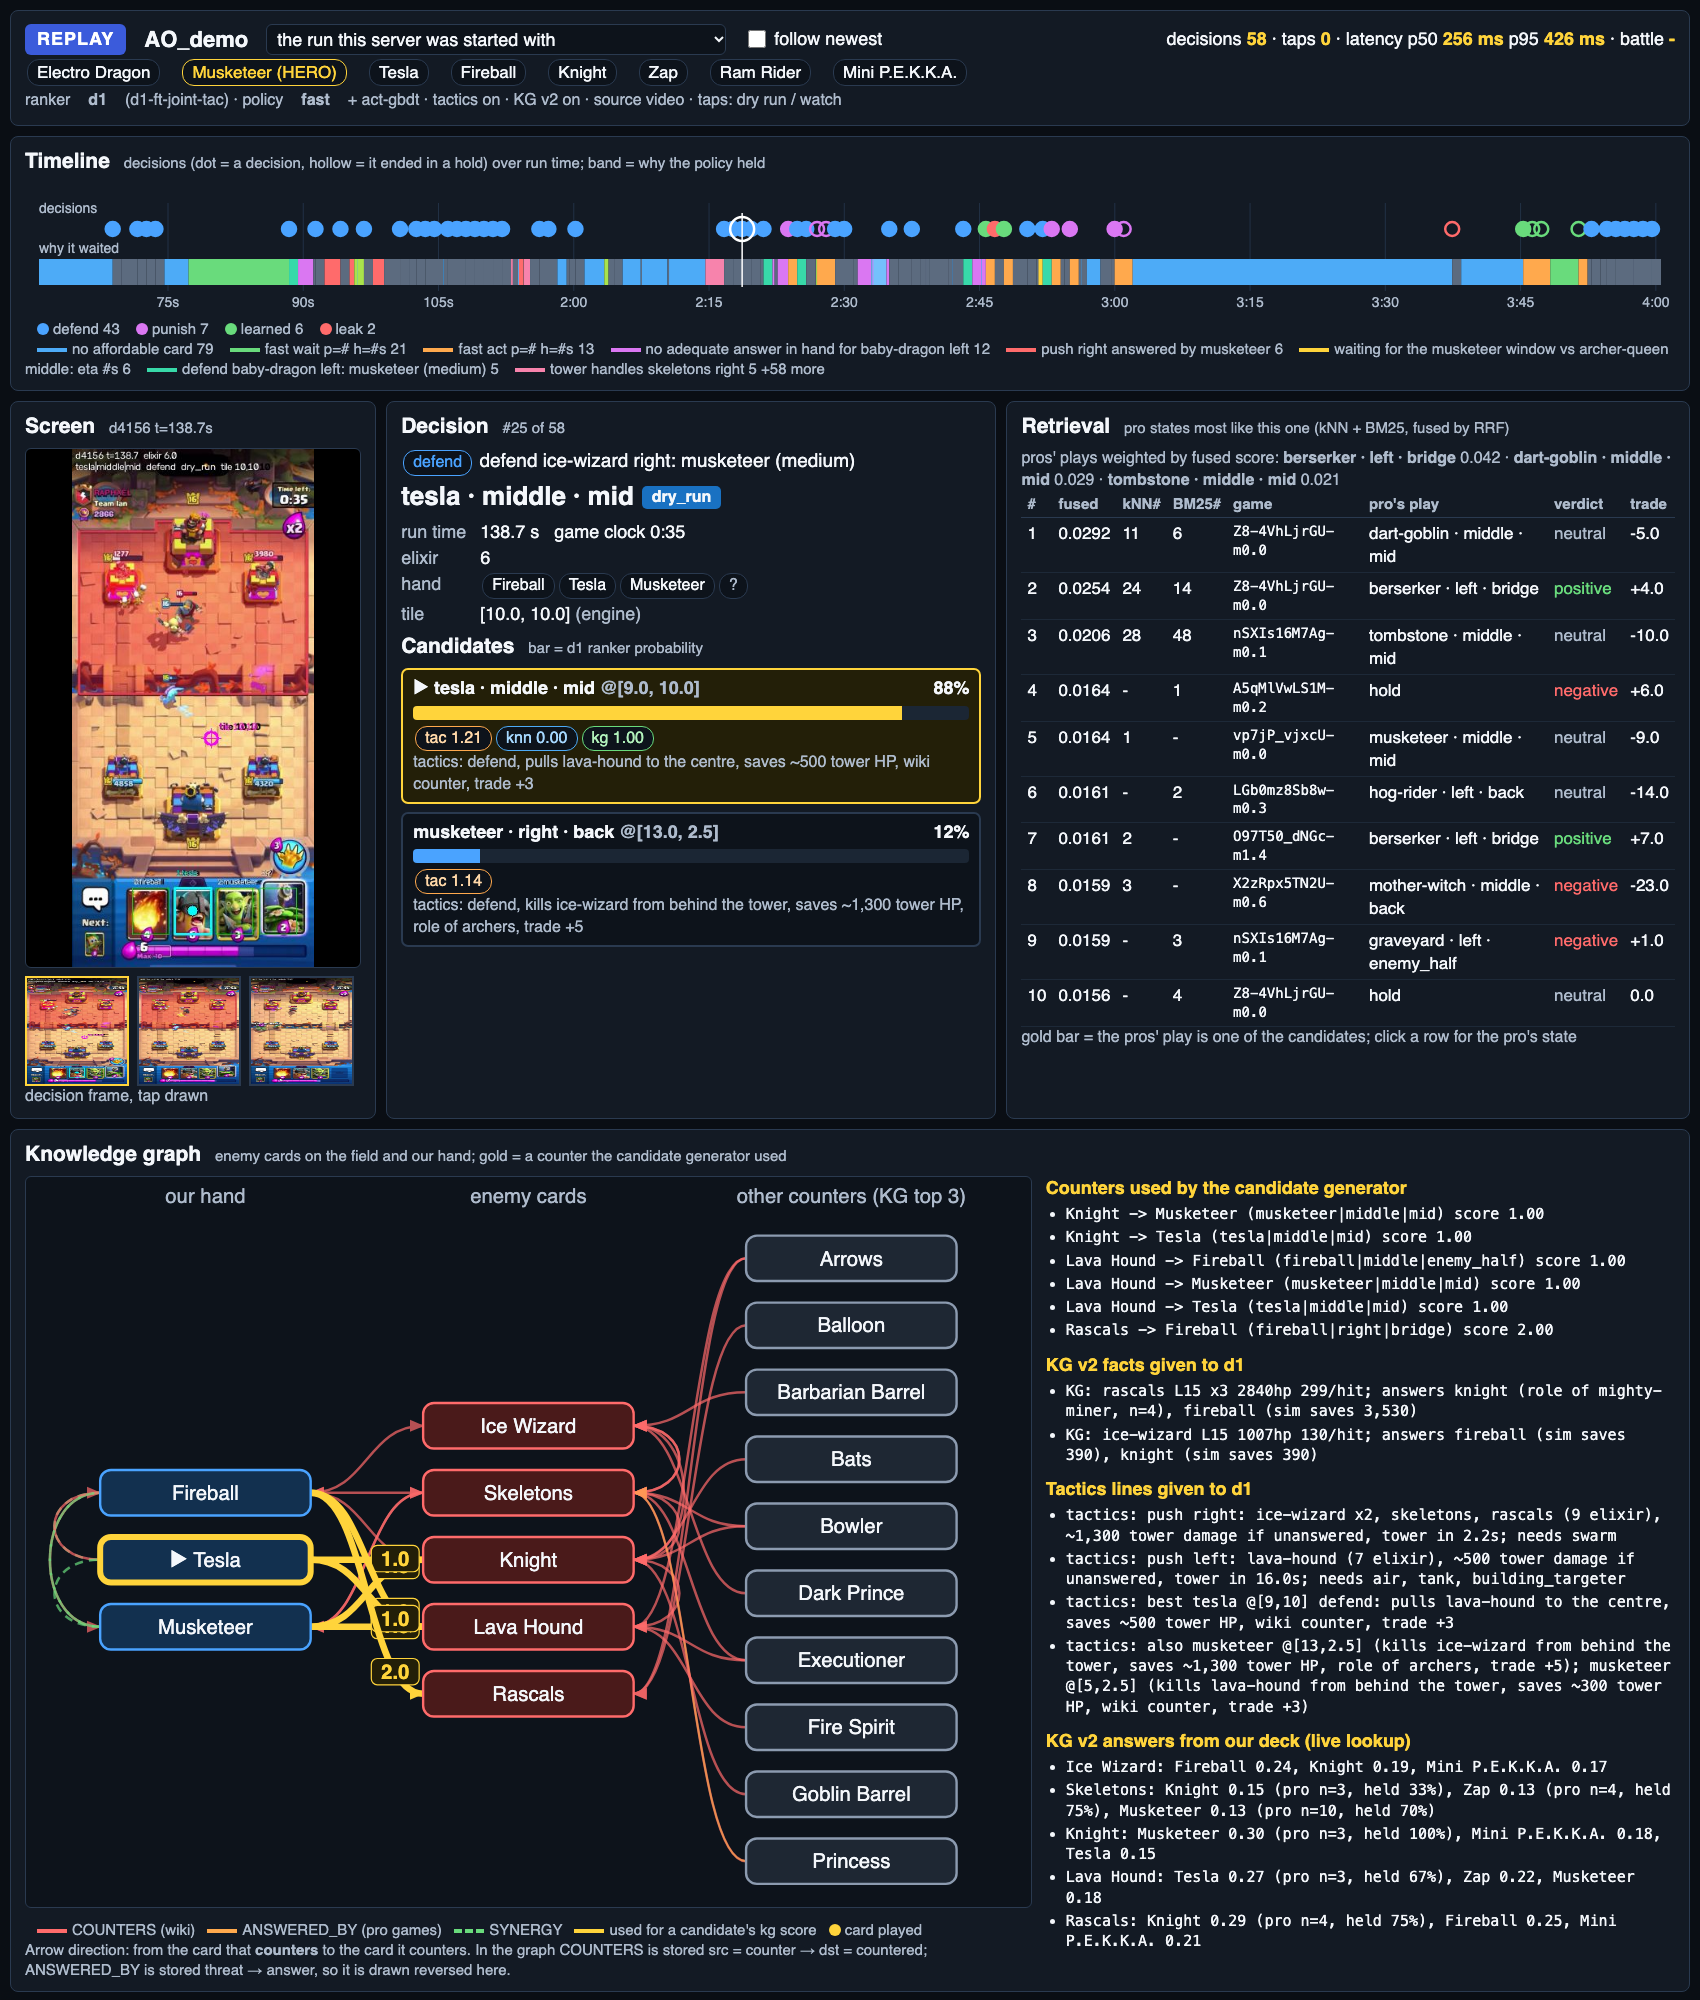
\includegraphics[width=\columnwidth]{figs/dashboard.png}
\caption{Decision dashboard on a video dry run. Top: timeline of decisions and hold reasons. Middle: decision frame; two candidates with d1 probabilities (Tesla 88\%) and the engine, kNN and KG scores behind them; the ten pro states retrieved by kNN+BM25 with RRF. Bottom: KG subgraph (our hand, enemy cards, counters used) and the \tw{KG:} and \tw{tactics:} lines d1 read.}
\label{fig:dashboard}
\end{figure}

% ---------------------------------------------------------------------------------------------
\section{Course Concepts in the System}
\label{sec:course}

Table~\ref{tab:course} maps each course block to what is built, where it runs and the number that tests it. Four course lessons recur in the results and are drawn together in Sec.~\ref{sec:disc}: tuned simple baselines are hard to beat~\cite{rendle2020ncfvsmf}; whether a model uses the knowledge in its context must be tested, not assumed~\cite{wu2024clasheval,ru2024ragchecker}; the evaluation protocol matters as much as the method (D-037, the equal-budget KGE audit~\cite{ruffinelli2020olddog}); and perception errors bound what the decision layer can do~\cite{huang2025esca}.

\begin{table*}[t]
\caption{Course techniques built into \cb{}. ``Live'' = on the default live path; ``off'' = offline evaluation or a flag only. Test split unless noted.}
\label{tab:course}
\centering\scriptsize
\setlength{\tabcolsep}{3pt}
\renewcommand{\arraystretch}{1.05}
\begin{tabular}{@{}L{2.0cm}L{4.1cm}L{4.95cm}L{5.0cm}l@{}}
\toprule
Block & Technique & Where in \cb{} & Evidence & Use\\
\midrule
Retrieval\newline L8--10~\cite{cap6938L08,cap6938L09,cap6938L10}
 & BM25~\cite{robertson2009bm25} + RRF ($k{=}60$)~\cite{cormack2009rrf} & FTS5 text channel fused with structured kNN & hit@10 0.160 fused vs 0.136 kNN alone & live\\
 & HNSW~\cite{malkov2020hnsw} vs exact search & index over 10,923 state vectors & ef 40: recall@10 0.978 at 0.31\,ms vs 1.51\,ms & off\\
 & Pre- vs post-filtering & deck and phase filters & deck pool empty for 88.9\% of queries; post@10 empty 50\%/87\% & off\\
 & Setwise LLM reranking~\cite{zhuang2024setwise,sun2023rankgpt} & d1 scores all ($\le$4) options in one pass & 0.507 fine-tuned vs 0.221 zero-shot (chance 0.25) & live\\
Dense repr.\newline L2--4~\cite{lim2026l02,lim2026l03}
 & Fixed-length vectors; small text embedder~\cite{xiao2023cpack} & 644-d hand-built vector; 384-d bge-small channel & text channel adds $\sim$20\,ms, hit@10 0.143: not integrated & live / off\\
RAG\newline L11--12~\cite{lim2026l11,lim2026l12}
 & Parametric-memory limit~\cite{mallen2023popqa}; retrieved context & engine, retrieval and KG notes in d1's context & zero-shot d1 at chance; accuracy vs key popularity (Fig.~\ref{fig:popularity}) & live\\
 & Distractor training (RAFT)~\cite{zhang2024raft} & 1 gold + 3 hard options on a 2$\times$2 grid & option-key shortcut 0.852 $\rightarrow$ 0.250 & train\\
 & Graph facts in context (GraphRAG)~\cite{edge2024graphrag} & up to 3 \tw{KG:} lines per decision & retrain on them: $-$2.2 pts [$-$4.7, +0.5] & live\\
 & Adaptive trigger~\cite{jiang2023flare,jeong2024adaptiverag} & play/wait gate decides when d1 is consulted & LightGBM bal.\ acc.\ 0.607 vs rules 0.509 ($h{=}2$\,s) & live\\
 & Abstention scoring (CRAG)~\cite{yang2024cragbench} & hold when d1's top probability $<$ 0.483 & utility 0.104 vs 0.013 answering all & off\\
Rec.\ systems\newline L13--14~\cite{lim2026l13,lim2026l14}
 & LM as recommender, full fine-tune~\cite{bao2023tallrec,geng2022p5} & d1-omni-600M, 313.6M trainable parameters & val/test 0.547/0.507 & live\\
 & Feature rankers~\cite{wang2021dcnv2,burges2010lambdamart}; tuned baselines~\cite{rendle2020ncfvsmf} & logreg, LambdaRank, DCN-V2 on 783 features & d1 $-$ LightGBM: +2.5 pts [$-$1.4, +5.9] & off\\
 & Sequential rec.\ (SASRec)~\cite{kang2018sasrec} & opponent next-card prediction & acc@1 0.222 vs copy-frequency 0.243 & off\\
KG\newline L5--7~\cite{cap6938L05,cap6938L06C,cap6938L07}
 & Typed KG feeding decisions & v1 590/12,030; v2 840/27,112, 19 relations & opp.-deck recall 0.234 vs popularity 0.130 ($k{=}1$) & live\\
 & KGE~\cite{bordes2013transe,yang2015distmult,trouillon2016complex,sun2019rotate}, audit protocol~\cite{ruffinelli2020olddog,sun2020reevaluation} & held-out COUNTERS triples, PyKEEN~\cite{ali2021pykeen} & RotatE MRR 0.159 vs popularity 0.110 & off\\
 & Rule mining with support~\cite{lajus2020amie3,liu2022tlogic} & 287 ``threat $\rightarrow$ pro answer'' rules (8\,s window) & hit@1 0.154 vs popularity 0.169, random 0.128 & live\\
 & Temporal copy mechanism~\cite{zhu2021cygnet} & copy-frequency next card; PLAYED\_AFTER edges & acc@1 0.243, beats SASRec & off\\
 & Neuro-symbolic hard constraints (L7) & legality filter, safety rules, lane simulation & pros' own play legal on 0.542--0.597 of states & live\\
Agents\newline L15--16~\cite{lim2026l15,lim2026l16}
 & Agent with tools~\cite{yao2023react}; one decision LLM & engine, retrieval, KG propose, d1 decides (D-045) & 13 runs, 931 logged decisions, 746 taps & live\\
 & Guarded execution; trajectory-level evaluation~\cite{yao2025taubench} & two-switch guard, banner gate, per-decision logs; open loop vs the pro & taps landed 75/84, 78/95; trial 0/10 wins; pro plays met $\pm$2\,s 77.1\% (null 68.9\%) & live\\
Knowledge upd.\newline L17--18~\cite{lim2026l17,lim2026l18}
 & Editing criteria~\cite{yao2023editingsurvey}; non-parametric edit~\cite{mitchell2022serac} & patch-versioned fact store & reliability 1.000; portability 1.000 vs 0.067 & off\\
 & Knowledge conflicts~\cite{wu2024clasheval,xie2024chameleon}; CAD/AdaCAD~\cite{shi2024cad,wang2025adacad} & down-weight pre-patch hits; corrupted notes (E2); contrastive decoding & 0.124 $\rightarrow$ 0.002; poisoned-note follow-rate 0.044, accuracy $-$0.4 pts; CAD no gain & off\\
\bottomrule
\end{tabular}
\end{table*}
% src (Table course): retrieval_ablation_v1.md (0.160, 0.136, 0.978, 0.31, 1.51, 88.9%, 50%/87%, 0.143); SA sec. 1/2/4 (0.507, 0.221, 0.547, -2.2, +2.5, 0.104/0.013); D-037 (0.852);
%   act_gbdt_v2.md (0.607 vs 0.509); CMA A2 (313.6M), A3 (0.542-0.597), C2, C6; next_card_v1.md (0.222, 0.243); opp_model_v1.md (0.234 vs 0.130);
%   kge_link_prediction_v1.md (0.159, 0.110); answer_rules_v1.md (0.154, 0.169, 0.128); BM sec. 11 (75/84, 78/95); edit_eval_v2.md = edit_eval_v1.md;
%   CC replicate joint_tac_v2, test (C3 follow-rate 0.044, delta -0.004; CAD a tuned on val = 0); VP headline (77.1%, null 68.9%); TRIAL (0/10)

% ---------------------------------------------------------------------------------------------
\section{Experiments}
\label{sec:exp}

\subsection{Setup}
Offline numbers come from the frozen decision code (D-051, commit \tw{66917e7}); outputs that predated code changes were re-run. Ranker evaluations use 761 val and 766 test lines from 26 and 27 held-out games. CIs are percentile intervals from 10,000 cluster-bootstrap resamples of whole games (seed 20261107), paired across models; we also give exact McNemar $p$, which treats lines as independent and is therefore the optimistic test. Thresholds, ensemble weights and feature-ranker configurations are chosen on val, so test is the clean column. % src: BM header; SA header

\subsection{Ranking the pro's play}
\label{sec:ranker}

\begin{table}[t]
\caption{4-way pick-the-pro-play accuracy (chance 0.25) with 95\% cluster-bootstrap CIs. ``Notes'' = tactics lines and per-option notes.}
\label{tab:ranker}
\centering\scriptsize
\setlength{\tabcolsep}{3pt}
\begin{tabular}{@{}lll@{}}
\toprule
Model & Val & Test\\
\midrule
\multicolumn{3}{@{}l}{\emph{Leak check and simple baselines}}\\
option-key rule, old options / 2$\times$2 grid & 0.853 / 0.250 & 0.852 / 0.250\\
random & 0.230 [0.207, 0.254] & 0.252 [0.218, 0.284]\\
popularity of the key & 0.468 [0.412, 0.516] & 0.325 [0.280, 0.374]\\
placement prior & 0.493 [0.430, 0.547] & 0.384 [0.337, 0.431]\\
\multicolumn{3}{@{}l}{\emph{Feature rankers, 783 features (seed 0)}}\\
logistic regression & 0.543 [0.492, 0.586] & 0.470 [0.423, 0.512]\\
LightGBM LambdaRank & 0.565 [0.520, 0.604] & 0.482 [0.448, 0.515]\\
\quad mean $\pm$ sd over 3 seeds & 0.5484 $\pm$ 0.0140 & 0.4913 $\pm$ 0.0126\\
DCN-V2 & 0.537 [0.493, 0.576] & 0.403 [0.366, 0.439]\\
\multicolumn{3}{@{}l}{\emph{d1-omni-600M decision LLM}}\\
zero-shot & 0.258 [0.226, 0.287] & 0.221 [0.191, 0.252]\\
ft-joint, plain lines & 0.524 [0.483, 0.561] & 0.483 [0.442, 0.522]\\
ft-joint, given notes it never saw & 0.477 [0.427, 0.523] & 0.461 [0.418, 0.506]\\
\textbf{ft-joint-tac} (trained on notes; live) & \textbf{0.547} [0.503, 0.584] & \textbf{0.507} [0.472, 0.540]\\
ft-joint-kg (also trained on \tw{KG:} lines) & 0.530 [0.480, 0.572] & 0.484 [0.450, 0.518]\\
\bottomrule
\end{tabular}
\end{table}
% src (Table ranker): SA sec. 1 (all CI rows); D-037 (0.853/0.852); feature_ranker_v2.md = feature_ranker_v1.md (3-seed mean); BM sec. 1 (option-set 0.250)

Table~\ref{tab:ranker} gives the main result. (1)~Zero-shot d1 is at chance (0.258/0.221): the 600M model has no usable Clash Royale knowledge, the parametric-memory limit discussed in~\cite{mallen2023popqa,lim2026l11}. (2)~Fine-tuning lifts it to 0.547/0.507, 12.3 points above the placement prior on test (CI [+8.0, +16.7], $p<0.001$). (3)~The tuned feature ranker matches the LLM: d1-ft-joint-tac minus LightGBM is +2.5 [$-$1.4, +5.9] (McNemar $p=0.263$), and against LightGBM's seed~2 it is $-$0.3 [$-$4.9, +4.0]. LightGBM's top features by gain are the option key's popularity (0.178) and $p(\text{zone}\mid\text{card})$ (0.124), the same priors as the simple baselines. % src: SA sec. 2; feature_ranker_v2.md (gain 0.1782, 0.1240)
(4)~Training on the tactics notes makes the model robust to them, not reliant on them. A model that never saw notes is hurt by them (0.461 vs 0.483 on test), and on the same lines the model trained with notes beats it by +4.6 [+1.0, +8.4] ($p=0.006$); but its gain over the no-notes model on that model's own plain lines, +2.3 [$-$0.9, +5.3], is not significant, and deleting the notes from its input does not lower its accuracy (Sec.~\ref{sec:conflict}). % src: SA sec. 2 (+4.6, +2.3); CC replicate (C1)
(5)~Retraining with \tw{KG:} lines did not help ($-$2.2 [$-$4.7, +0.5] against d1-ft-joint-tac): validation loss rose from 1.1916 to 1.6708 in the second epoch, and the KG facts on training lines are mined from the same pro games, a leak we have not removed. % src: SA sec. 2; CMA C4 (val loss); CMA A2 RETRO row (FIX_LIST #49)

\begin{figure}[t]
\centering
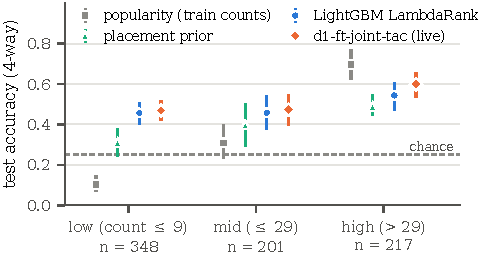
\includegraphics[width=\columnwidth]{figs/fig_popularity.pdf}
\caption{Test accuracy by training frequency of the gold key (terciles; 95\% cluster-bootstrap CIs). Popularity wins on head keys and fails on the tail; the fine-tuned LLM and LightGBM hold up on rare keys. Data: \tw{stats\_audit\_v1.json}.}
\label{fig:popularity}
\end{figure}

Fig.~\ref{fig:popularity} splits test accuracy by how often the gold key occurs in training. Popularity alone is the best model on head keys (0.696) and the worst on the tail (0.103); d1-ft-joint-tac and LightGBM stay level across the two lower terciles (0.468/0.473 and 0.457/0.458), so both generalise beyond memorised keys. A share of 0.14 of test gold keys never occurs in training. % src: SA sec. 5

d1 is well calibrated (test ECE 0.048 over 15 bins; Brier 0.616), so its probability can drive abstention. Holding when the top probability is below 0.483 (chosen on val) answers 0.402 of test lines at 0.630 accuracy and raises the +1/0/$-$1 utility of CRAG-style scoring~\cite{yang2024cragbench} from 0.013 [$-$0.056, 0.079] to 0.104 [0.060, 0.147] (Fig.~\ref{fig:retsel}b). A d1+LightGBM ensemble fitted on val changes test accuracy by $-$0.1, +2.1 or +3.9 points depending on LightGBM's seed, so we do not claim it; a rule arbiter that narrows d1's options when d1 is unsure gives no gain either (0.509 vs 0.506), so it stays off. % src: SA sec. 3, 4, 6; arbiter_v2.md (50.6% / 50.9%)

\subsection{Retrieval}
\label{sec:retr}

\begin{table}[t]
\caption{Retrieval channels (val n = 916 / test n = 902 queries, train pool, depth 50). Hit@10: the pro's exact play is among the top-10 neighbours' plays.}
\label{tab:retrieval}
\centering\scriptsize
\setlength{\tabcolsep}{3.5pt}
\begin{tabular}{@{}lccc@{}}
\toprule
List & hit@10 val / test & card hit@10 val / test & ms p50 (test)\\
\midrule
BM25 (FTS5) & 0.142 / 0.159 & 0.396 / 0.483 & 25.8\\
structured kNN (644-d) & 0.166 / 0.136 & 0.434 / 0.412 & 2.1\\
text (bge-small, 384-d) & 0.132 / 0.143 & 0.397 / 0.436 & 22.2\\
struct + BM25 (live) & 0.138 / 0.160 & 0.434 / 0.487 & 28.0\\
all three, RRF & 0.156 / 0.170 & 0.461 / 0.514 & 49.6\\
\bottomrule
\end{tabular}
\end{table}
% src (Table retrieval): docs/data/retrieval_ablation_v1.md (kept current per BM sec. 3)

Table~\ref{tab:retrieval}: the channels are within noise of each other (test hit@10 0.136--0.170), and BM25 beats the structured channel on test (0.159 vs 0.136) but not on val. The text channel adds about 20\,ms per query for no clear gain, so the live list is structured plus BM25. As a candidate source alone, kNN voting loses to popularity on exact keys (test recall@10 0.317 vs 0.402) and wins only on cards (0.651 vs 0.607). % src: CMA A1 (ranker_baselines_v1.json candidate_recall)
HNSW at ef 40 keeps recall@10 at 0.978 in 0.31\,ms against 1.51\,ms for exact search (Fig.~\ref{fig:retsel}a); at 10.9k vectors exact search is affordable, so the live path uses it. Filtering shows the pre- versus post-filter trade-off from the indexing lecture~\cite{cap6938L09}: a deck pre-filter leaves an empty pool for 88.9\% of queries (their decks never occur in training), and post-filtering the top 10 returns nothing for 50.0\% (deck) and 87.3\% (phase) of queries; post-filtering the top 200 brings this down to 0.5\% and 0.1\%. % src: retrieval_ablation_v1.md (HNSW table, filtering table)

\begin{figure}[t]
\centering
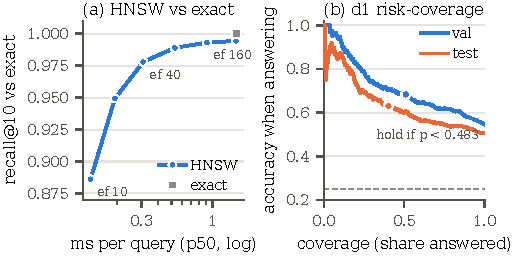
\includegraphics[width=\columnwidth]{figs/fig_retrieval_selective.pdf}
\caption{(a) HNSW recall@10 against exact kNN versus query time (10,923 vectors, $k{=}10$). (b) Risk--coverage of d1-ft-joint-tac when it holds below a probability threshold; dots: 0.483, chosen on val.}
\label{fig:retsel}
\end{figure}

\subsection{Knowledge graph: embeddings and mined rules}
\label{sec:kg}

\begin{table}[t]
\caption{(a) Held-out COUNTERS link prediction, test (762 queries, filtered, 3 seeds). (b) Ranking the pro's own deck for a held-out threat (E6); rules mined from training games only.}
\label{tab:kg}
\centering\scriptsize
\setlength{\tabcolsep}{3.5pt}
\begin{tabular}{@{}lccc@{}}
\toprule
\multicolumn{4}{@{}l}{(a) KG embeddings} \\
Method & MRR & H@1 & H@10\\
\midrule
random & 0.0223 & 0.0113 & 0.1129\\
popularity & 0.1103 & 0.0381 & 0.2385\\
TransE & 0.0819 $\pm$ 0.0046 & 0.0000 & 0.2380\\
DistMult & 0.0907 $\pm$ 0.0083 & 0.0232 & 0.1986\\
ComplEx & 0.1162 $\pm$ 0.0074 & 0.0367 & 0.2616\\
RotatE & \textbf{0.1588} $\pm$ 0.0020 & 0.0713 & 0.3259\\
\midrule
\multicolumn{4}{@{}l}{(b) Mined answer rules (609 val / 433 test events)} \\
Score & hit@1 val & hit@1 test & MRR test\\
\midrule
full \tw{KG2.answers\_for} & 0.182 & 0.154 & 0.374\\
pro-mined rules only & 0.191 & 0.129 & 0.350\\
wiki COUNTERS only & 0.117 & 0.141 & 0.359\\
train popularity of the answer card & 0.182 & 0.169 & 0.384\\
random card in deck (expected) & 0.126 & 0.128 & 0.345\\
\bottomrule
\end{tabular}
\end{table}
% src (Table kg): (a) docs/data/kge_link_prediction_v1.md (setting full); (b) docs/data/answer_rules_v1.md headline val/test tables

\emph{Link prediction} (Table~\ref{tab:kg}a). We hold out wiki COUNTERS triples (3,043/380/381) and rank 126 candidate cards with filtered, tie-aware ranks. All four PyKEEN~\cite{ali2021pykeen} models get the same grid (dimension 32 or 64, learning rate 0.01 or 0.001), chosen on val MRR, and three seeds, following the course's evaluation-audit protocol~\cite{ruffinelli2020olddog,sun2020reevaluation,cap6938L05}. RotatE~\cite{sun2019rotate} is best (MRR 0.1588, H@10 0.3259) and beats popularity (0.1103); TransE (0.0819) and DistMult (0.0907) do not. DistMult is symmetric by construction (asymmetry score 0.0), while only 940 of 3,804 counter pairs have a reverse edge. % src: CMA A3 (triples, grid, asymmetry, 940 / 3,804); kge_link_prediction_v1.md

\emph{Mined answer rules} (E6, Table~\ref{tab:kg}b). For each held-out event we rank the pro's own deck (7.96/7.83 cards on average) with rules mined from training games (support $\ge3$, 8\,s window). Pooled over val and test, the full score beats random (+0.044 hit@1, CI [+0.020, +0.068]) and the wiki counters (+0.043 [+0.011, +0.074]) but not the training popularity of the answer card ($-$0.006 [$-$0.035, +0.020]); on test the pro-mined source alone falls below popularity ($-$0.040 hit@1, $p=0.022$). The score barely predicts whether the answer held the tower (AUROC 0.543), few rules have large support (best support 10 or more for 63 of 1,042 events), and the 8\,s window is the best of 2, 4 and 8\,s on val (MRR 0.409). AMIE and TLogic score rules on the data they were mined from~\cite{lajus2020amie3,liu2022tlogic}; held out, our 287 rules look useful against random and the wiki counters but not against the popularity baseline the KGE audit protocol asks for~\cite{ruffinelli2020olddog}, which suggests they mostly re-encode how often the pro plays each card: a weak prior~\cite{cap6938L07}. % src: answer_rules_v1.md (paired val+test, test paired, AUROC, strata, sweep)

\subsection{Context conflict: does d1 follow wrong notes? (E2)}
\label{sec:conflict}

Following ClashEval and the knowledge-conflict lecture~\cite{wu2024clasheval,xie2024chameleon,lim2026l17}, we corrupt d1-ft-joint-tac's context without changing the gold label: C1 removes the notes and the \tw{tactics:}/\tw{KG:} lines, C2 shuffles the notes across options, C3 swaps the gold option's informative note with a distractor's and names a wrong card in the \tw{tactics:} line (relevant but misleading), and C4 transplants the tactics/KG block of another line (irrelevant). Follow-rate is the share of movable lines (the corruption favours an option d1 did not already pick) whose pick moves to the favoured option.

Table~\ref{tab:conflict}: no condition moves accuracy by more than 1.2 points (all McNemar $p\ge0.27$). Removing the whole context changes 21\% of picks, but gains and losses cancel (57 vs 56 lines); poisoned notes move 4.4\% [2.1, 6.8] of movable picks. Lines whose gold option carries the informative note are easier than lines where a distractor's does (0.564 vs 0.371), but the gap persists with no notes at all (0.599 vs 0.401), so it reflects which states are easy, not d1 reading the notes. Context-aware decoding~\cite{shi2024cad}, which contrasts the scores with and without context, selects weight $a=0$ on val in every condition, and each $a>0$ lowers test accuracy on C0 by 1.7 to 2.9 points; AdaCAD's adaptive weight~\cite{wang2025adacad} averages 0.014 and changes accuracy by $-$0.1 points. % src: CC replicate joint_tac_v2 (test tables, strata, CAD C0)
d1 thus avoids both failures the course warns about, adopting wrong context over its prior (ClashEval~\cite{wu2024clasheval}) and greater sensitivity to relevant-but-misleading than to irrelevant noise (RAGChecker~\cite{ru2024ragchecker}), because it barely reads its notes. One plausible reason is in the data: the notes favour the gold option on only 30\% of test lines and a distractor on 22\% (49\% have none), so discounting them costs little. The result makes d1 robust to wrong tool output and explains why retraining on \tw{KG:} lines did not help (Sec.~\ref{sec:ranker}). % src: CC replicate test note status (227 right, 167 wrong, 372 none of 766)

\begin{table}[t]
\caption{Context conflict on d1-ft-joint-tac (E2), test lines (n = 766, 27 games), 95\% cluster-bootstrap CI; $p$ = exact McNemar; follow-rate as in the text (C4: 12 movable lines).}
\label{tab:conflict}
\centering\scriptsize
\setlength{\tabcolsep}{3.5pt}
\begin{tabular}{@{}lllcc@{}}
\toprule
Condition & Accuracy [CI] & $\Delta$ pts ($p$) & Changed & Follow\\
\midrule
C0 as exported & 0.507 [0.473, 0.539] & -- & -- & --\\
C1 context removed & 0.508 [0.476, 0.541] & +0.1 (1.00) & 21\% & --\\
C2 notes shuffled & 0.517 [0.482, 0.550] & +1.0 (0.27) & 7\% & 0.094\\
C3 notes poisoned & 0.503 [0.469, 0.535] & $-$0.4 (0.76) & 6\% & 0.044\\
C4 block transplanted & 0.495 [0.459, 0.530] & $-$1.2 (0.45) & 19\% & 0.083\\
\bottomrule
\end{tabular}
\end{table}
% src (Table conflict): docs/data/context_conflict_v1.md, replicate on joint_tac_v2 (HEAD notes, same lines as Table III), "Accuracy by condition - test" and "Follow-rate - test"; p = exact McNemar

\subsection{When to act}

\begin{table}[t]
\caption{Play/wait timing on dense test seconds (n = 5,279): balanced accuracy for ``the pro deploys within $h$''.}
\label{tab:timing}
\centering\scriptsize
\setlength{\tabcolsep}{4pt}
\begin{tabular}{@{}lccc@{}}
\toprule
Policy & $h$ = 1\,s & $h$ = 2\,s & $h$ = 3\,s\\
\midrule
hand-written rules & 0.506 & 0.509 & 0.510\\
LightGBM, 29 features & 0.594 & \textbf{0.607} & 0.613\\
\quad AUC & 0.632 & 0.659 & 0.672\\
rules + LightGBM (live \emph{fast}) & 0.571 & 0.584 & 0.593\\
\bottomrule
\end{tabular}
\end{table}
% src (Table timing): docs/data/act_gbdt_v2.md overview + apples-to-apples test table; act_head_v2.md (0.558, unchanged from v1)

Table~\ref{tab:timing}: LightGBM reaches balanced accuracy 0.607 (AUC 0.659) at $h=2$\,s against 0.509 for the hand-written rules, and the live combination, in which rules override the model in four modes, sits between them (0.584). On the balanced subset ($h=1$\,s, n = 3,221) used to train a d1 act head (top 8 layers, 168.9M trainable parameters), LightGBM scores 0.598 against the head's 0.558, at 0.05\,ms instead of about 70\,ms per call: a second case where the tuned simple model beats the LLM. % src: act_gbdt_v2.md (apples-to-apples test table); act_head_v2.md (0.558); CMA B (act head 168.9M, ~70 ms), C4

\subsection{Next card, opponent deck and knowledge editing}

Opponent next-card prediction is a sequential recommendation task~\cite{kang2018sasrec,lim2026l14}. SASRec (3 seeds) reaches acc@1 0.129/0.222 on val/test and loses to a copy-frequency rule (0.207/0.243), the copy intuition of CyGNet~\cite{zhu2021cygnet,cap6938L06C}; popularity is near zero (0.000/0.002) because opponents vary, and the ceiling set by cards already seen is 0.678/0.644. The KG-based opponent-deck model recovers hidden cards with recall 0.234/0.291/0.327 after 1/2/3 seen cards, against 0.130/0.124/0.118 for popularity (leave-one-game-out, 155 games). % src: next_card_v1.md; opp_model_v1.md (BM sec. 7)
For knowledge editing~\cite{yao2023editingsurvey,lim2026l17} we apply a synthetic +1-elixir patch to five cards in a patch-versioned fact store, the non-parametric route of SERAC~\cite{mitchell2022serac}: reliability, generalisation and portability are 1.000 (0.000, 0.000 and 0.067 without the edit), locality is 1.000, rollback passes, and re-weighting cuts retrieved hits that use an edited card from 0.124 to 0.002. The store is deterministic, so this shows that the mechanism works, not that it generalises to a real balance patch~\cite{yang2025mirage}. % src: edit_eval_v2.md (identical to edit_eval_v1.md)

\subsection{Bot versus pro on the pros' own videos}

We run the full live stack open loop on held-out (test-split) pro videos with the pro's deck and a dry-run executor, and match the bot's would-be taps to the pro's plays within $\pm$2\,s. Open loop means the bot's taps do not change the video: this measures what the bot would do in the pro's situation, not whether it would win, and its hand memory is never told that a card left the hand. Retrieval uses only train and val games; the KG answers and placement prior come from train games. The results cover all 24 usable test games (90\,min of video, 1,561 pro plays, 2,042 bot taps); four more have an incomplete deck. % src: VP header and "Not run" list

Table~\ref{tab:vspro}. \emph{Timing:} 77.1\% of pro plays have a bot tap within 2\,s (a median 0.47\,s away), against 68.9\% for a null that shifts the bot's own taps by 20--60\,s, which matters because the bot taps more often than the pro (22.8 vs 17.4 times per minute) and spends more elixir (58.7 vs 33.6 per minute). \emph{Choice:} the bot picks the pro's card on 17.1\% of matched pairs, against 12.8\% for a random card of its perceived hand; where a KG threat exists it scores 19.8\% against 15.6\% for the KG v1 counter rule. The ceiling bounds the gap: the pro's card is in the bot's perceived hand on only 40.1\% of plays (53.0\% in the offline read), and the bot cannot pick a card it does not see. Missed pro plays were most often held because no card was affordable (23.0\%), the engine judged that the tower handles the push (22.7\%) or the act model waited (18.8\%). % src: VP Headline, Timing (0.47 s; elixir/min 58.72, 33.58), When the bot held

\begin{table}[t]
\caption{Bot vs pro on held-out pro videos, open loop: 24 test games, 1,561 pro plays. Percent; window $\pm$2\,s; 95\% CIs by game bootstrap. Null: the bot's own taps shifted by 20--60\,s. Baselines use the same plays; the placement prior is given the pro's card.}
\label{tab:vspro}
\centering\scriptsize
\setlength{\tabcolsep}{3pt}
\begin{tabular}{@{}lll@{}}
\toprule
Measure & Bot [95\% CI] & Baseline\\
\midrule
pro plays met by a bot tap & 77.1 [71.8, 83.0] & 68.9 (null)\\
bot taps met by a pro play & 72.6 [69.3, 76.2] & 67.9 (null)\\
taps (bot) / plays (pro) per min & 22.8 [20.2, 25.9] & 17.4 [16.5, 18.4]\\
same card, matched pairs & 17.1 [14.6, 20.2] & 12.8 (random in hand)\\
same card, KG threat exists (126) & 19.8 [13.3, 26.9] & 15.6 (KG v1 counter)\\
pro's card in perceived hand & 40.1 [37.3, 43.2] & 53.0 (dataset's hand)\\
same lane $\mid$ same card (103) & 42.7 [31.6, 53.5] & 44.6 (placement prior)\\
same key $\mid$ same card (103) & 26.2 [16.8, 36.0] & 29.7 (placement prior)\\
\bottomrule
\end{tabular}
\end{table}
% src (Table vspro): docs/data/vs_pro_v1.md (MAC-AQ, generated 2026-11-08T02:31:35Z, all 24 usable test games) Headline table (every cell, subset sizes 126 and 103) and Timing table.

\subsection{Live play and comparison with prior bots}
\label{sec:live}

\begin{table}[t]
\caption{(a) Decision latency by stage, ms p50 / p95: the live trial session (363 decisions), and the mean over 3 repeated video dry runs ($\pm$ sd for the total; a shared Mac, so upper bounds). (b) Live record in Training Camp.}
\label{tab:live}
\centering\scriptsize
\setlength{\tabcolsep}{3.5pt}
\begin{tabular}{@{}lcc@{}}
\toprule
\multicolumn{3}{@{}l}{(a) Stage \hfill trial session \quad dry run, 3 reps}\\
\midrule
capture & 22.0 / 44.8 & 0.8 / 4.3\\
perception (detector, OCR, hand) & 108.0 / 266.4 & 179.2 / 234.2\\
live state & 0.13 / 0.31 & 0.2 / 0.5\\
trigger (rules + LightGBM) & 1.1 / 9.2 & 2.7 / 9.7\\
candidates (engine, retrieval, KG) & 26.8 / 57.9 & 46.7 / 86.1\\
rank (d1; 0 when one candidate) & 0.0 / 140.9 & 87.1 / 191.0\\
execute (two clicks) & 181.0 / 188.8 & no clicks\\
\textbf{total} & \textbf{322.7 / 601.6} & 271.7$\pm$20.1 / 455.2$\pm$41.2\\
\midrule
\multicolumn{3}{@{}l}{(b) Live record}\\
\midrule
runs before the trial, 11-03 to 11-07 & \multicolumn{2}{l}{13 (12 live), 931 decisions, 746 taps}\\
taps landed, two newest of them & \multicolumn{2}{l}{75/84, 78/95 (older run 233907: 95/100)}\\
run 013441 (3 battles) & \multicolumn{2}{l}{tower taken; 3-crown loss; \textbf{win in overtime}}\\
\textbf{trial}: wins / battles, exact CI & \multicolumn{2}{l}{\textbf{0 / 10}, 95\% CI 0--30.8\%}\\
\quad crowns for / against (10 battles) & \multicolumn{2}{l}{3 / 18; a tower taken in 3; 2 in overtime}\\
\quad per logged battle (9 of 10) & \multicolumn{2}{l}{40.3 decisions, 27.0 taps; median 213\,s}\\
\bottomrule
\end{tabular}
\end{table}
% src (Table live): (a) trial-session column: LOG decisions.jsonl timings_ms, all 363 rows, nearest-rank p50 / p95 (total 322.7 / 601.6);
%   dry-run column: LAT "Whole stack, 3 repeated dry runs" (video Z8-4VhLjrGU 60-180 s, runs/rerun/lat_{1,2,3}), mean of p50 / p95, sd for total
%   (b) CMA C6 = BM sec. 13 (12 live runs, 931, 746) + LAT (dry run 20261105-205720); BM sec. 11 (tap_landing_20261107-013441_v2.md 75/84,
%   tap_landing_20261107-111554_v2.md 78/95, tap_landing_233907_v1.md 95/100); STATUS 2026-11-07 night (run 013441);
%   trial rows: TRIAL (0/10, scores, crowns 3/18, 2 OT, 3 with a tower; Clopper-Pearson 0-30.8%, checked with scipy beta.ppf(0.975,1,10) = 0.3085);
%   LOG battles.jsonl (9 TRAINING_CAMP rows: 363 decisions, 243 taps, median duration 212.6 s) and decisions.jsonl timings_ms (total 323/602)

Before the trial, thirteen recorded runs between 2026-11-03 and 2026-11-07 (12 live, one dry) logged 931 decisions, of which 746 sent a tap. Their total latency is 347/613\,ms p50/p95 (339/572\,ms in run 111554). In the trial session (Table~\ref{tab:live}a) perception (108\,ms p50) and the two-click execute stage (181\,ms) dominate; d1 adds nothing at the median, because most decisions have a single candidate, and 141\,ms at p95. The 300\,ms p95 target was missed in every live run and in all three dry runs. Failed taps concentrate on Tesla (11 of 19 landed in run 111554) and Fireball (3 of 7); run 013441 brought the first win, in overtime. % src: CMA C6, C7 (347/613; 338.9/571.8 run 111554); LOG (trial session); LAT (dry runs: 0 of 3 meet the target); BM header (shared Mac); tap_landing_20261107-111554_v2.md (tesla 11/19, fireball 3/7); STATUS 2026-11-07 night
\emph{Trial.} On 2026-11-07 ten Training Camp battles were played through the launcher (\tw{scripts/demo.sh --live}) on the frozen code (D-051), with results recorded by hand. The bot lost all ten (Table~\ref{tab:live}b): 0--1 five times (once in overtime), 0--2, 0--3, 1--2 and 1--3 twice (once in overtime), 3 crowns for and 18 against. The exact 95\% CI for its win rate is 0--30.8\%, and against KataCR's 1/20 a two-sided Fisher exact test gives $p=1.0$: no detectable difference. The session log holds 9 of the 10 battles (one battle start was missed), and the banner gate correctly refused two non-battle screens whose banner read ``2618''. % src: TRIAL (scores, Fisher p = 1.0 checked with scipy fisher_exact [[0,10],[1,19]]); LOG (decisions.jsonl timings_ms; battles.jsonl n = 2, 3 banner "2618" NOT_TRAINING_CAMP)

\begin{table}[t]
\caption{Prior Clash Royale agents and \cb{}. R = reported by the authors, M = measured by us. Protocols differ; see text.}
\label{tab:prior}
\centering\scriptsize
\setlength{\tabcolsep}{2pt}
\begin{tabular}{@{}L{1.3cm}L{2.25cm}L{1.95cm}L{2.4cm}@{}}
\toprule
 & KataCR~\cite{wu2025nonembedded} & Claude Royale~\cite{houseworth2025claudeRoyale} & \cb{} (ours)\\
\midrule
Interface & phone video stream, ADB taps (Linux) & BlueStacks on macOS & iPhone Mirroring on macOS, Quartz clicks\\
Perception & YOLOv8-l$\times$2 (mAP 67.4), OCR, ResNet classifiers & Claude vision on screenshots & KataCR's YOLOv8 weights, OCR, Kalman tracker\\
Decision maker & offline-RL StARformer & Claude Haiku, 3 player agents & gate + engine + retrieval + KG; fine-tuned 600M LLM picks\\
Knowledge used at inference & none (in weights) & hand-written prompts and notes & 10,923 pro states, KG v1/v2, tactics engine\\
Training data & 105 episodes, 113,981 frames, one player vs AI & none (prompting) & 197 pro games, 33 videos\\
Latency & 120\,ms decision + 240\,ms fusion (R) & $\sim$7\,s per agent (R) & 323 / 602\,ms p50 / p95, capture to click, trial session (M)\\
Offline decision metric & none & card choice 11/25 on labelled screenshots (R) & 4-way test accuracy 0.507 (M)\\
Opponent & built-in AI, Training Camp & human ladder & built-in AI, Training Camp\\
Win rate vs built-in AI, 95\% CI & 1/20 = 5\% [0.1, 24.9]; 0--10\% over 9 models (R) & none (ladder; not comparable) & trial 0/10 [0, 30.8]; one earlier win (M)\\
\bottomrule
\end{tabular}
\end{table}
% src (Table prior): PBC sec. 0, 1.2-1.4, 2.1-2.2, 4, 5 (Clopper-Pearson 1/20: 0.1-24.9%); ours CMA C7, SA sec. 1; TRIAL (0/10, CI, Fisher); STATUS 2026-11-07 night (earlier win)

Table~\ref{tab:prior}: only KataCR and \cb{} report a win rate against the built-in AI, and even there protocols differ: KataCR played the 2024 game (Season 59) with another deck, and its 1/20 is the best of ten epochs selected on the same 20 games, an optimistic estimate. KataCR's latency excludes actuation; ours includes it. We reuse KataCR's detector and do not claim a better one. % src: PBC sec. 5, 6

% ---------------------------------------------------------------------------------------------
\section{Discussion and Limitations}
\label{sec:disc}

Four results are negative for the system we set out to build; each repeats a lesson from the course.

\emph{Tuned simple baselines match the LLM.} LightGBM is within 2.5 points of d1 (not separable); on timing it beats a fine-tuned d1 act head (0.598 vs 0.558) at 0.05 instead of about 70\,ms; and copy-frequency beats SASRec. Well-tuned simple models often match neural ones~\cite{rendle2020ncfvsmf,lim2026l13}, and 197 games from one creator leave a 600M model little to learn beyond the priors a GBDT reads directly. % src: SA sec. 2; feature_ranker_v2.md; act_gbdt_v2.md; next_card_v1.md
\emph{d1 does not read its context} (Sec.~\ref{sec:conflict}). ClashEval and RAGChecker study models that follow their context too readily~\cite{wu2024clasheval,ru2024ragchecker}; d1 sits at the other extreme. With the engine near chance as a ranker (4-way 0.293/0.265 val/test), the tools contribute by proposing candidates, not by writing notes~\cite{lim2026l13}. % src: CC replicate; tactics_eval_v2.md
\emph{Mined rules approximate popularity} (Sec.~\ref{sec:kg}). The evaluation audits the course teaches~\cite{ruffinelli2020olddog,sun2020reevaluation} ask for exactly this baseline; the same habit caught the option-set leak before d1 was fine-tuned on it (D-037). % src: D-037 (2026-11-02) precedes D-039 (fine-tune go-ahead, 2026-11-03)
\emph{Perception caps agreement with the pro.} The pro's card is in the bot's perceived hand for only 40.1\% of plays; the pro's own move is legal under our reading on only 0.542--0.597 of states; and in an early live run 14 of 27 decisions were skipped because the hand read as unknown. As the ESCA lecture argues, perception errors dominate embodied-agent failures~\cite{huang2025esca,cap6938L06C}: no ranker can choose a card the bot does not see. % src: VP headline (40.1); CMA A3 (0.542-0.597); BM sec. 13 and PBA 2.2 (14 of 27; CMA A3 says 15 of 27)

\emph{Why the trial was lost (limitations and future work).} The trial log shows decisions built on bad perception, the ESCA pattern again~\cite{huang2025esca}. (1)~\emph{Tower HP.} OCR drops digits, so one tower read 4424$\leftrightarrow$424 seven times in 30\,s, and a fallen tower reads unknown, not 0, so the larger deploy area it opens was never used, although a tower fell in 3 battles. (2)~\emph{No committed target.} Counter-pushes follow the lane of the defended push, so damage is split (one battle ended with the enemy towers at 1,663 and 1,824 HP, neither taken), and after a tower fell ram riders kept taking its lane, i.e.\ went at the king. (3)~\emph{No support} troop is ever offered behind a surviving defence or a ram rider. (4)~\emph{Spell value.} Fireball is valued by elixir destroyed, not tower damage prevented, so none was proposed against a bunched Giant, Balloon and Bats push, and the Zap group rule counts tanks. (5)~\emph{Over-playing:} 27 taps per battle, 40 emergency defends at 2--5 elixir and 30 tap pairs under 1.6\,s apart; on video the bot taps 22.8 times per minute to the pro's 17.4, and ``no affordable card'' is its top reason for missing a pro play. (6)~\emph{Phantom threats:} a stationary ``Graveyard'', a card the trainer's deck lacks, triggered defences six times. All six sit in the hand-written engine and policy, the components our benchmarks rate lowest (rules 0.509 balanced accuracy on timing, the engine 0.265 as a ranker): the untuned-baseline lesson~\cite{rendle2020ncfvsmf}. d1 cannot repair them, as it ranks only when two or more candidates survive (119 of 279 executed plays) and does not read the notes. The fixes (a monotone HP filter, a per-battle target tower, pocket placements, support moves, spell value from prevented damage, an elixir budget at the pro's rate) are specified for a re-run against this 0/10 baseline. % src: BL W1 (B1 4424/424 x7, t 41-70), W3 (legal_zones needs 0), W2 (B4 1663/1824; B8 ram riders right after the right tower fell), W4, W5 (B9 giant+balloon+bats, value by elixir), W6 (group rule counts the giant), W8 (243 taps / 9 battles; 40 emergency defends 2-5 elixir), W9 (30 pairs < 1.6 s), W10 (graveyard x6, not in Trainer Cheddar's deck); VP (22.8 vs 17.4; "no affordable card" 23.0%); act_gbdt_v2.md (0.509); tactics_eval_v2.md (0.265); CMA sec. 0 (119/279)

\emph{Other limitations.} d1's serve-time context carries a \tw{[plan]} line that no training line contains, a train/serve mismatch we have not measured. Every offline number rests on 26--27 held-out games (CIs about $\pm$3.5 points) from one creator, and three of our eight cards have no pro plays at all, so the engine and role transfer carry them. Video evaluation is open loop, the perception does not read enemy health bars (units are simulated at full HP), and a larger d1-2B fine-tune (val 0.4192) was never tested because its checkpoint failed to load. Trial results were recorded by hand: the end-of-battle frames missed the result screen in 5 of 9 battles. % src: CMA sec. 0 ([plan]); SA sec. 1 (26/27 games); CGA sec. 7.3 E1 and PBA 2.4 (about +/-3.5 pts at n = 766); D-047 (ram-rider, electro-dragon, mini-pekka have no pro plays); STATUS MAC-AM merged (#57 full HP); CMA C4 (d1-2B 0.4192, load crash); BL W11 (5 of 9)

% ---------------------------------------------------------------------------------------------
\section{Conclusion}

\cb{} shows that a non-embedded agent can play Clash Royale live on a laptop, with knowledge-graph, retrieval and simulation tools feeding a fine-tuned LLM that keeps the final say, at 323\,ms from capture to click (trial session). It does not yet beat Training Camp reliably: it won one battle in an early session and lost all ten battles of the trial (95\% CI 0--30.8\%, no different from KataCR's 1/20), because it misreads tower HP, commits to no target tower, values spells by elixir and over-plays. The benchmarks give a partly negative picture: fine-tuning turned a chance-level LLM into one that picks the pro's play half the time, but tuned simple models match or beat it at most sub-tasks, it does not read the notes the tools write for it, the mined rules re-encode popularity, and on pro video its card choice is capped by perception. Next steps: fix those four failures and re-run the 10-battle trial with automatic result logging, measure perception against labelled frames, and train d1 on lines where notes and leak-free KG facts carry signal the state lines do not. Code, tests, benchmark files (\tw{docs/data/BENCHMARKS.md}) and the decision log are in the project repository. % src: CMA C7; SA sec. 1; CC; AR; VP; PBA 2.5; TRIAL; BL (suggested order, W11)

\bibliographystyle{IEEEtran}
\bibliography{refs}

\end{document}
